

\subsection{Melihat Daftar Kupon}
Halaman ini hanya dapat diakses oleh \textit{administrator} yang sebelumnya sudah \textit{login}. Detail kasus penggunaan dapat dilihat Tabel \ref{uc06.03}.\\
\indent Tidak ada \textit{view logic} ataupun logika \textit{UI} khusus dalam halaman ini. Kode sumber implementasi \textit{back-end} dapat dilihat pada Kode Sumber \ref{cdbe.06-02}.

  \begin{figure}[H]
  	\centering
  	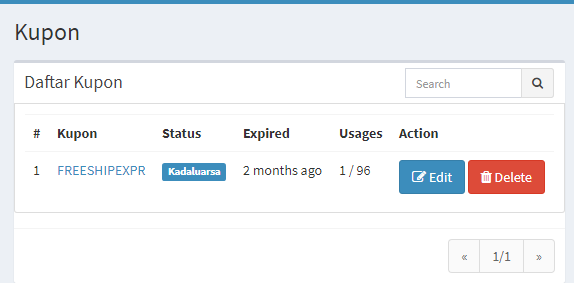
\includegraphics[width=\textwidth]{images/bab4/ui/06-02.png}
  	\caption{Halaman Antarmuka Kasus Penggunaan Melihat Daftar Kupon}
  	\label{ui.06-02}
  \end{figure}
\begin{lstlisting}[label=cdbe.06-02,style=php,caption=Implementasi Antarmuka Melihat Daftar Kupon]

/** File : app/Http/Controllers/CouponController
 * Menampilkan halaman daftar kupon
 * tidak terkait dengan CouponRepository
 * langsung diFetch dari base Model Coupon
 * Method : GET
 */

public function index()
{
    $data['data'] = Coupon::orderBy('activedate', 'desc')->paginate(20);
    return view('pages.coupon.index', $data);

}
\end{lstlisting}
      

      
